\documentclass{article}

\usepackage{arxiv}

\usepackage{iftex}

\ifPDFTeX
  \usepackage[utf8]{inputenc}
  \usepackage[T1]{fontenc}
\else
  \usepackage{fontspec}
  \setmainfont{Times New Roman}
  \setsansfont{Arial}
  \setmonofont{Courier New}
\fi

\usepackage{hyperref}
\usepackage{url}
\usepackage{booktabs}
\usepackage{amsfonts}
\usepackage{amsmath}
\usepackage{nicefrac}
\usepackage{microtype}
\usepackage{enumitem}
\usepackage{graphicx}
\usepackage{natbib}
\usepackage{doi}
\usepackage{float}

\usepackage{caption}
\usepackage{cleveref}

\captionsetup{font=small,labelfont=bf,skip=4pt}
\setlist{nosep,leftmargin=*}

\title{PaddleOCR-VL-Circuit: Built for Schematic Diagram Understanding}

\newif\ifuniqueAffiliation
\uniqueAffiliationtrue

\ifuniqueAffiliation
\author{ Jianning Zhang \\
    School of Flexible Electronics\\
    Sun Yat-sen University\\
    Shenzhen, Guangdong, China \\
    \texttt{zhangjn83@mail2.sysu.edu.cn} \\
    \And
    Yifei Chen \\
    School of Computer Science\\
    Sun Yat-sen University\\
    Guangzhou, Guangdong, China \\
    \texttt{chenyf376@mail2.sysu.edu.cn} \\
}
\else
\usepackage{authblk}
\renewcommand\Authfont{\bfseries}
\setlength{\affilsep}{0em}
\newbox{\orcid}\sbox{\orcid}{
\includegraphics[scale=0.06]{orcid.pdf}}
\author[1]{%
    \href{https://orcid.org/0000-0000-0000-0000}{\usebox{\orcid}\hspace{1mm}Jianning Zhang\thanks{\texttt{zhangjn83@mail2.sysu.edu.cn}}}%
}
\author[2]{%
    \href{https://orcid.org/0000-0000-0000-0000}{\usebox{\orcid}\hspace{1mm}Yifei Chen\thanks{\texttt{chenyf376@mail2.sysu.edu.cn}}}%
}
\affil[1]{School of Flexible Electronics, Sun Yat-sen University, Shenzhen, China}
\affil[2]{School of Computer Science, Sun Yat-sen University, Guangzhou, China}
\fi

\renewcommand{\headeright}{}
\renewcommand{\undertitle}{}
\renewcommand{\shorttitle}{PaddleOCR-VL-Circuit}

\hypersetup{
pdftitle={PaddleOCR-VL-Circuit: Built for Schematic Diagram Understanding},
pdfsubject={Circuit Schematic OCR, Visual Language Model, LoRA Fine-tuning},
pdfauthor={Jianning Zhang, Yifei Chen},
pdfkeywords={Circuit Schematic, OCR, PaddleOCR-VL, LoRA, Netlist Extraction},
}

\date{}

\begin{document}
\maketitle

\begin{abstract}
Automatic recognition of circuit schematic diagrams is a core challenge in Electronic Design Automation (EDA). This technical report presents CircuitOCR, a system based on PaddleOCR-VL-0.9B for circuit schematic OCR and netlist extraction. We construct the V5 Golden dataset of 1,857 schematics (500 synthetic + 1,357 real KiCad projects) with 100\% visual-literal alignment. Through systematic LoRA ablation experiments, we identify the root cause of modality collapse---fine-tuning the vision-language projector destroys pre-trained alignment---and introduce the LLM-Only LoRA strategy that resolves it. The V10-Fixed model uses wide LoRA ($r=16$, $\alpha=32$, 5.7M params), fixes three critical training bugs (causal token double-shift, BPE boundary merging, \texttt{set\_state\_dict} silent failure in Paddle 3.1.0), and trains for 3 epochs (1,165 steps) in 43 minutes on an RTX 4060 (8\,GB). Phase 1 multi-metric evaluation on easy50-pure (44 samples) yields Component F1 = 0.2061 (4.5$\times$ over baseline 0.0455), Token Recall = 0.1540 (96$\times$ over baseline 0.0016), and NED = 0.8031 (baseline 0.9296, 13.6\% relative error reduction). S600 is the optimal checkpoint; S800 overfits (RepRate 40.9\%). All code, weights, datasets, and a live demo are open-sourced.
\end{abstract}

\keywords{Circuit Schematic \and OCR \and PaddleOCR-VL \and LoRA Fine-tuning \and Netlist Extraction \and Modality Collapse}


\section{Introduction}

Vision-Language Models (VLMs) can directly output structured text from images end-to-end, but their application to circuit schematic diagrams remains unexplored. No dedicated public benchmark exists for circuit schematic OCR. Existing datasets like Open Schematics~\citep{openschematics2025} lack standardized evaluation protocols, while textbook-derived datasets suffer from SPICE-induced visual-to-logic annotation discrepancies.

The industrial need is substantial. The global semiconductor market exceeded \$600 billion in 2025 (SEMI/WSTS). PCB reverse engineering outsourcing alone exceeds \$500 million annually, with approximately 30\% of time spent on schematic reconstruction. Use cases include hardware reverse engineering, legacy document digitization (1980s--2000s paper schematics), cross-tool migration, and the 500,000+ KiCad/EAGLE projects on GitHub lacking structured netlist exports.

Circuit schematic understanding involves two heterogeneous sub-tasks: (1) visual text recognition---extracting component designators (R1, C1), values (10k, 100nF), and net labels (VCC, GND); (2) topology graph tracing---inferring electrical connectivity from wires and net labels. Our evaluation protocol measures both dimensions: text NED for explicit recognition and component F1 for implicit structural understanding.


\section{System Setup}

We adopt PaddleOCR-VL-0.9B~\citep{cui2025paddleocrvl} (908M params), which integrates a NaViT-style dynamic vision encoder with the ERNIE-4.5-0.3B language model, supporting 109 languages. The unfine-tuned base model fails systematically on circuit schematics: it outputs generic document text (e.g., parameter tables), memorized hallucinations, or repetitive token sequences. These failures stem from pre-training data dominated by general documents with negligible exposure to engineering drawings.


\section{V5 Golden Dataset}

\subsection{Legacy Issues and Design Principles}

Earlier dataset versions (V1--V4) had three fatal flaws: (1) GT-image misalignment---labels from KiCad S-expression parsing included invisible pin numbers and hidden net names; (2) format mismatch---Open Schematics subsets used horizontal space-concatenated format (62.1\% single-word lines vs.\ test set's 98.6\%); (3) duplication noise---22,340 intra-line duplicate word pairs contaminating 24.3\% of samples.

V5 Golden was rebuilt on two principles: (1) GT must align 100\% with visible on-image text, using \texttt{draw.text()} synchronous recording for synthetic data and SVG stroked-text extraction for real KiCad data, with zero AI-generated labels; (2) format must match the test set, replacing mismatched subsets with train-real data (97.9\% single-word lines), reducing duplication noise by 99.5\% (22,340 $\to$ 107).

\subsection{Data Sources and Statistics}

\textbf{Synthetic V3 (500 images).} Random circuit topologies (5--30 components, 10 types) rendered as PNG, with labels from \texttt{draw.text()} logs~\citep{zhang2026circuitocr}.

\textbf{train-real (1,357 images).} Real open-source KiCad projects from GitHub, rendered via kicad-cli SVG $\to$ cairosvg PNG, with GT from SVG stroked-text visible elements in one-word-per-line vertical format.

\begin{figure}[h]
\centering
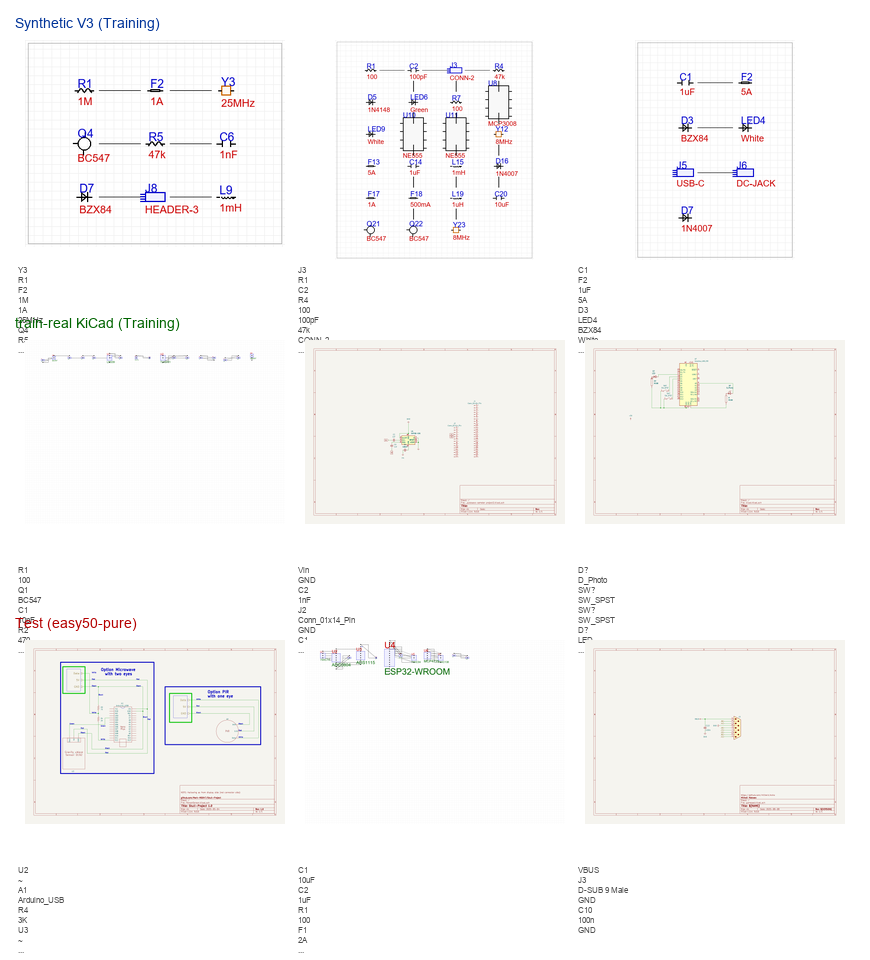
\includegraphics[width=\textwidth]{../circuit-ocr-dataset/figures/dataset_overview.png}
\caption{Dataset overview: three data sources. \textbf{Top row}---Synthetic V3: programmatically generated with randomized topologies (5--30 components, 10 types), GT recorded synchronously via \texttt{draw.text()}. \textbf{Middle row}---train-real (KiCad): real open-source projects from GitHub, rendered via kicad-cli SVG$\to$cairosvg PNG, GT extracted from SVG stroked-text. \textbf{Bottom row}---Test set (easy50-pure): held-out real schematics for evaluation. All images are raw PNG renders with zero AI-generated labels.}
\label{fig:dataset_overview}
\end{figure}

\begin{table}[h]
\centering
\caption{Dataset Composition and Split}
\label{tab:dataset}
\begin{tabular}{lcccc}
\toprule
\textbf{Split} & \textbf{Synthetic V3} & \textbf{train-real} & \textbf{Total} & \textbf{avg Lines} \\
\midrule
Training   & 450 & 1,104 & 1,554 & 32.1 \\
Validation & 50  & 171   & 171   & 33.4 \\
Test (easy50) & -- & --  & 44    & -- \\
Test (easy100) & -- & -- & 89   & -- \\
\midrule
\textbf{Total} & \textbf{500} & \textbf{1,357} & \textbf{1,857} & -- \\
\bottomrule
\end{tabular}
\end{table}

During training, we apply online augmentations: random JPEG compression (quality 85--100), random scaling (max\_dim 168--384px), and random horizontal flipping.


\section{Model Fine-Tuning}

\subsection{Modality Collapse: Discovery and Root Cause}

Initial full LoRA experiments ($r=8$, q/k/v/o self-attention, 2.75M params on 2,433 samples) reduced NED from 0.8848 to 0.8554, but output diversity collapsed to 4\%---nearly all test samples produced identical output. We define this as \textbf{Modality Collapse}.

Through six controlled experiments (E1--E6) summarized in Table~\ref{tab:ablation}, we systematically identified the root cause:

\begin{table}[h]
\centering
\caption{Ablation Experiments for Modality Collapse}
\label{tab:ablation}
\begin{tabular}{lcp{3cm}p{3cm}}
\toprule
\textbf{Exp} & \textbf{Variable} & \textbf{Result} & \textbf{Conclusion} \\
\midrule
E1 & Real vs.\ blank image & Outputs differ & Vision encoder works \\
E2 & Resolution 168$\to$336px & Still collapses & Resolution not the cause \\
E3 & 1 vs.\ 3 epochs & NED improves 0.9\% & Multi-epoch helps but insufficient \\
E4 & Add Projector LoRA & NED drops to 0.8271 & \textbf{Projector is the bottleneck} \\
E5 & Rank $r=8\to r=16$ & NED drops to 0.7961 & Capacity helps, diversity still 4\% \\
E6 & Freeze Projector & Diversity 90\% & \textbf{Collapse fully resolved} \\
\bottomrule
\end{tabular}
\end{table}

\textbf{Core finding: Projector LoRA is the root cause.} The vision-language projector (\texttt{mlp\_AR}, 25.9M params) is the sole bridge from visual features to language space. LoRA perturbation distorts these features into out-of-distribution vectors the LLM cannot interpret, causing it to degenerate into repeating high-frequency training tokens. Freezing the Projector while teaching only the LLM to reinterpret existing visual features is the safe strategy.

\subsection{V5: LLM-Only LoRA Validation}

V5 freezes the Projector and fine-tunes only LLM self-attention ($r=8$, $\alpha=16$, 1.25M params), with resolution increased to 384px and learning rate $2\times10^{-5}$. Training on 1,857 samples for 1 epoch (928 steps, 22 min) achieved 90\% output diversity---the first fine-tuned model to produce different outputs for different images. However, $r=8$ capacity was insufficient: NED (0.9031) remained below baseline due to premature convergence at $\sim$200 steps.

\subsection{V10-Fixed: Three Technical Fixes}

V10-Fixed scales LoRA to $r=16$, $\alpha=32$ (5.7M params, 0.63\% of 908M), targeting 310 projection matrices across LLM self-attention and linear layers. Three critical training bugs were fixed:

\begin{enumerate}[nosep]
    \item \textbf{Causal token double-shift}: PaddleOCR-VL's \texttt{AutoModelForConditionalGeneration} internally applies causal shift. Our manual shift caused double-shifting---supervising step $t$ with label $t+2$, corrupting gradients. Fixed by removing the manual shift.
    \item \textbf{BPE boundary merging}: Concatenating prompt and label strings before tokenization causes BPE to merge characters across the boundary (e.g., ``\texttt{\textbackslash n}'' + ``R'' $\to$ merged token). Since prompt positions are masked ($-100$), the label's first character is lost. Fixed by tokenizing prompt and label independently and concatenating token IDs.
    \item \textbf{\texttt{set\_state\_dict} silent failure}: In Paddle 3.1.0, \texttt{LoRAModel.set\_state\_dict()} returns \texttt{None} instead of a tuple, causing silent LoRA loading failure. Fixed by using the \texttt{LoRAModel} wrapper with manual \texttt{p.set\_value()} per parameter.
\end{enumerate}

Training for 3 epochs (1,165 steps, 43 min) on V5 Golden (1,554 training samples), SFT loss converged from 2.71 to 0.30.

\subsection{Phase 1 Multi-Metric Evaluation}

Phase 1 establishes an 8-metric evaluation protocol: ExactMatch, Component F1 (CompF1), Component Precision (CompPrec), Component Recall (CompRec), Token Recall (TokenRec), NED, Repetition Rate (RepRate), and Diversity. We evaluated all four checkpoints (S400, S600, S800, final) on easy50-pure (44 samples).

\begin{table}[h]
\centering
\caption{Phase 1 Multi-Metric Benchmark (easy50-pure, 44 samples)}
\label{tab:phase1}
\begin{tabular}{lcccccccc}
\toprule
\textbf{Model} & \textbf{ExactMatch} & \textbf{CompF1} & \textbf{CompPrec} & \textbf{CompRec} & \textbf{TokenRec} & \textbf{NED} $\downarrow$ & \textbf{RepRate} & \textbf{Diversity} \\
\midrule
Base   & 0\% & 0.0455 & 0.0455 & 0.0455 & 0.0016 & 0.9296 &  6.8\% & 90.9\% \\
S400   & 0\% & 0.1820 & 0.1862 & 0.2501 & 0.1302 & 0.8298 & 20.5\% & 95.5\% \\
\textbf{S600} & 0\% & \textbf{0.2061} & 0.2024 & \textbf{0.3114} & \textbf{0.1540} & \textbf{0.8031} & 15.9\% & 90.9\% \\
S800   & 0\% & 0.2080 & 0.2862 & 0.1996 & 0.1191 & 0.8063 & 40.9\% & 93.2\% \\
\bottomrule
\end{tabular}
\par\smallskip
{\small\noindent S600 is optimal. S800 overfits: RepRate surges to 40.9\% while TokenRec drops to 0.1191.}
\end{table}

\begin{figure}[H]
\centering
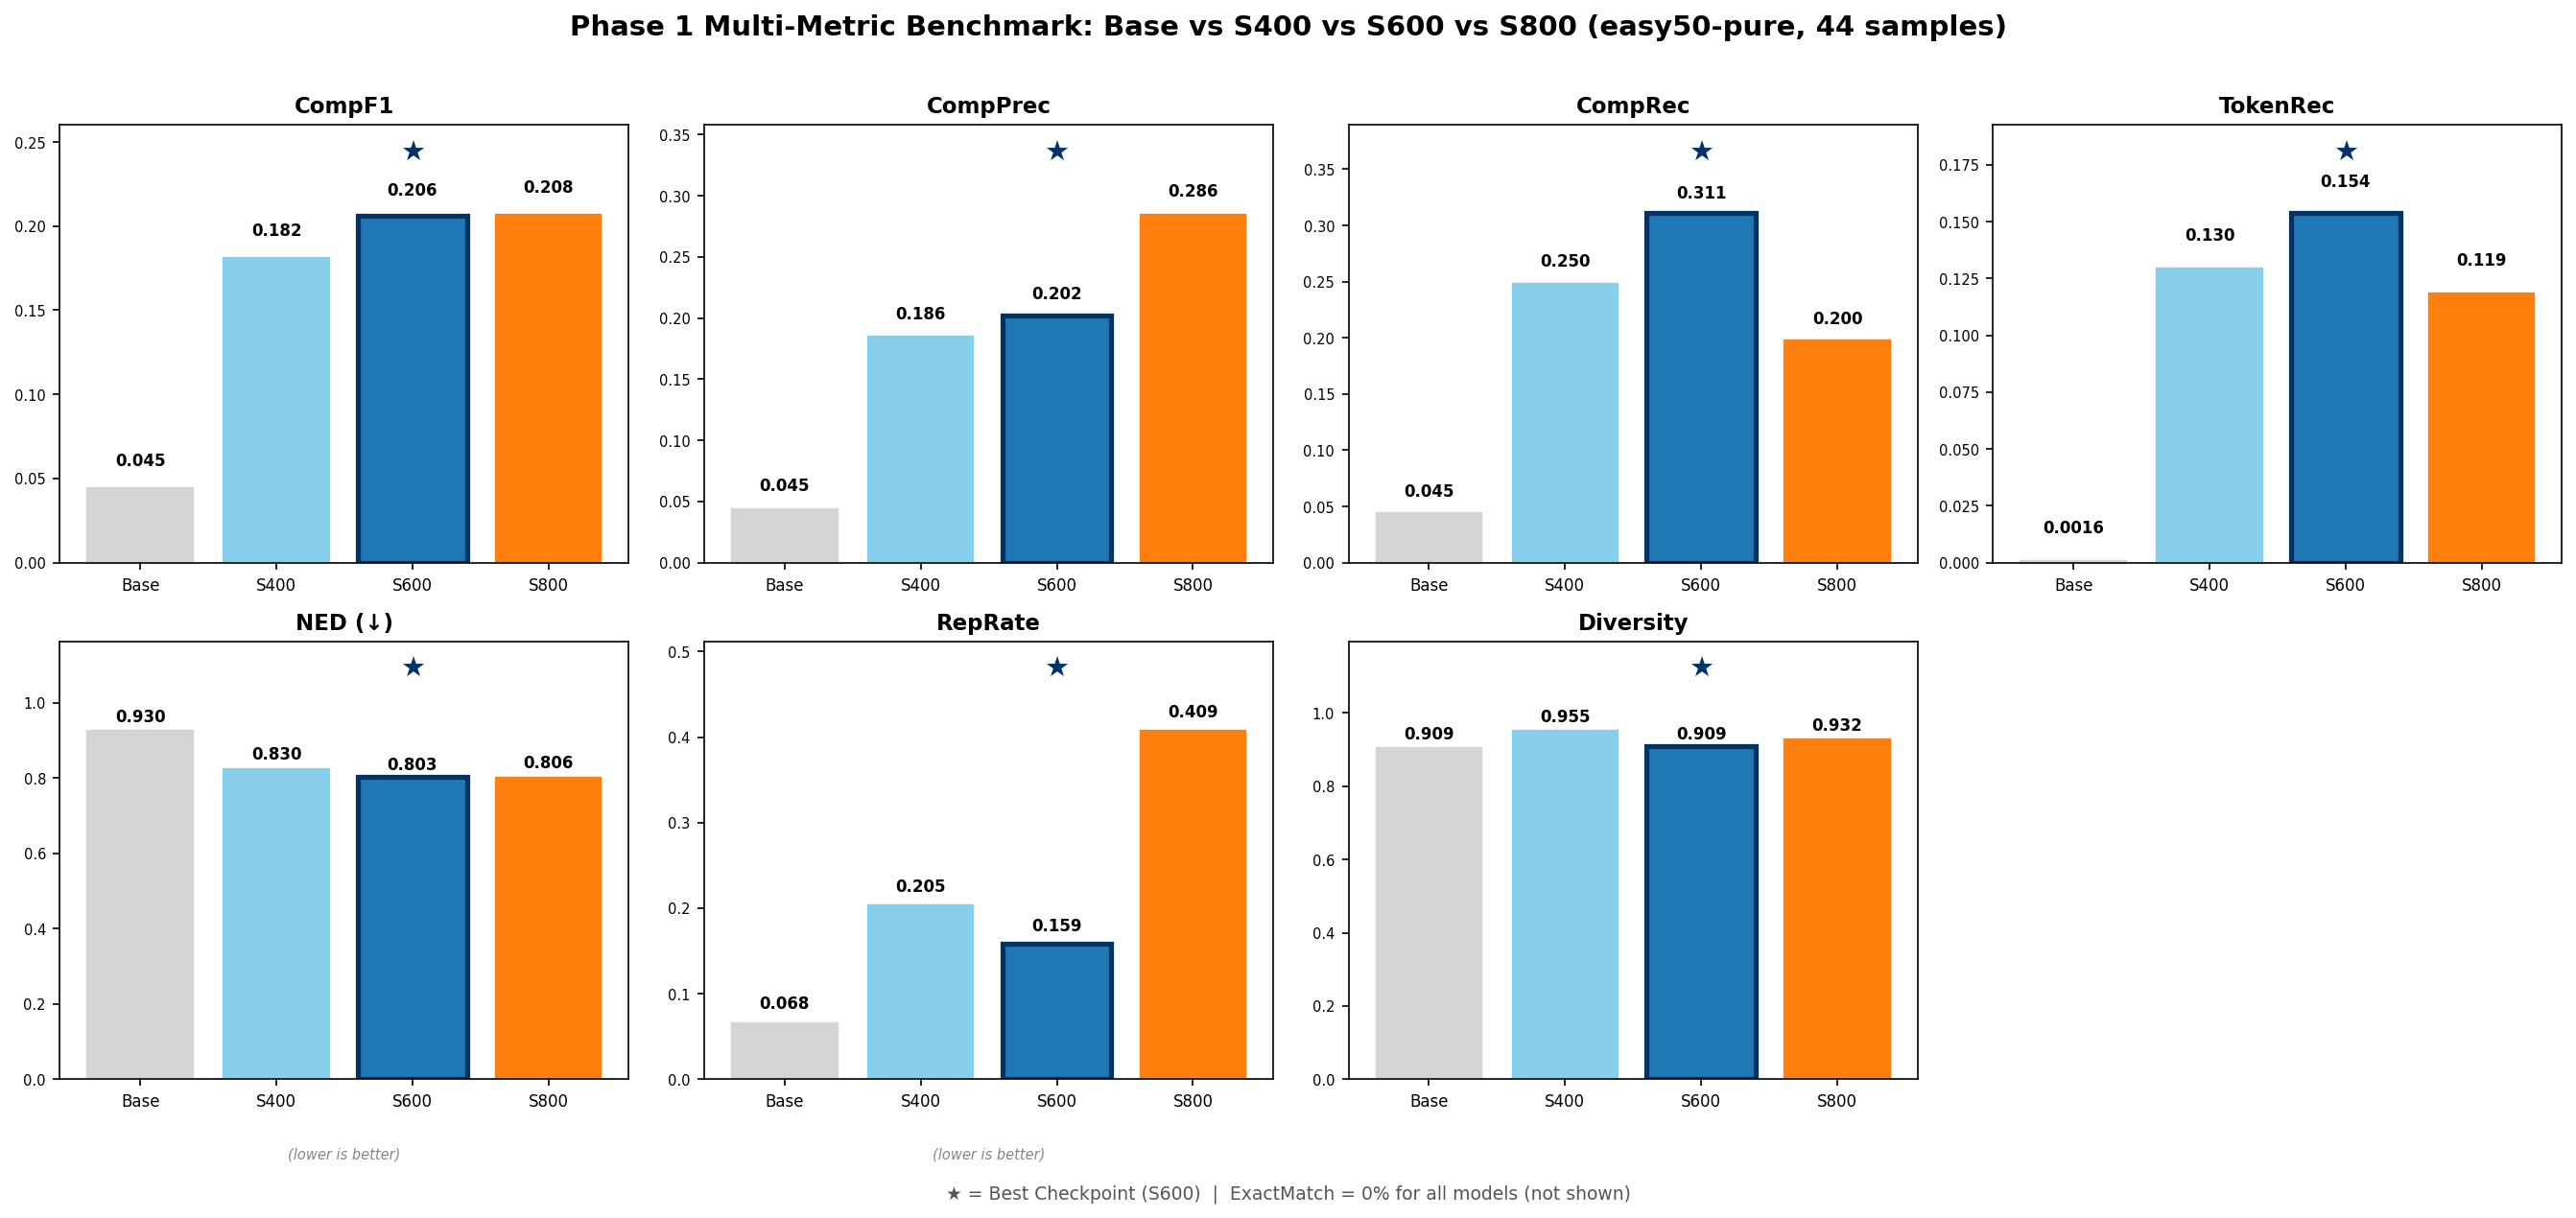
\includegraphics[width=\textwidth]{../circuit-ocr-dataset/figures/phase1_metrics_chart.png}
\caption{Phase 1 benchmark visualization across seven metrics (ExactMatch omitted: 0\% for all). S600 (blue, starred) achieves the best balance. S800 (orange) shows clear overfitting.}
\label{fig:phase1_chart}
\end{figure}

Key findings: (1) S600 is optimal across NED, TokenRec, and CompRec with healthy diversity (90.9\%). (2) S800 overfits: RepRate 40.9\% (nearly 3$\times$ S600), CompRec collapses to 0.1996. (3) CompF1 improves 4.5$\times$ (0.0455 $\to$ 0.2061), TokenRec 96$\times$ (0.0016 $\to$ 0.1540). (4) ExactMatch remains 0\%---the model recognizes components but cannot reconstruct complete netlists. (5) No modality collapse: all checkpoints exceed 90\% diversity.

\begin{figure}[h]
\centering
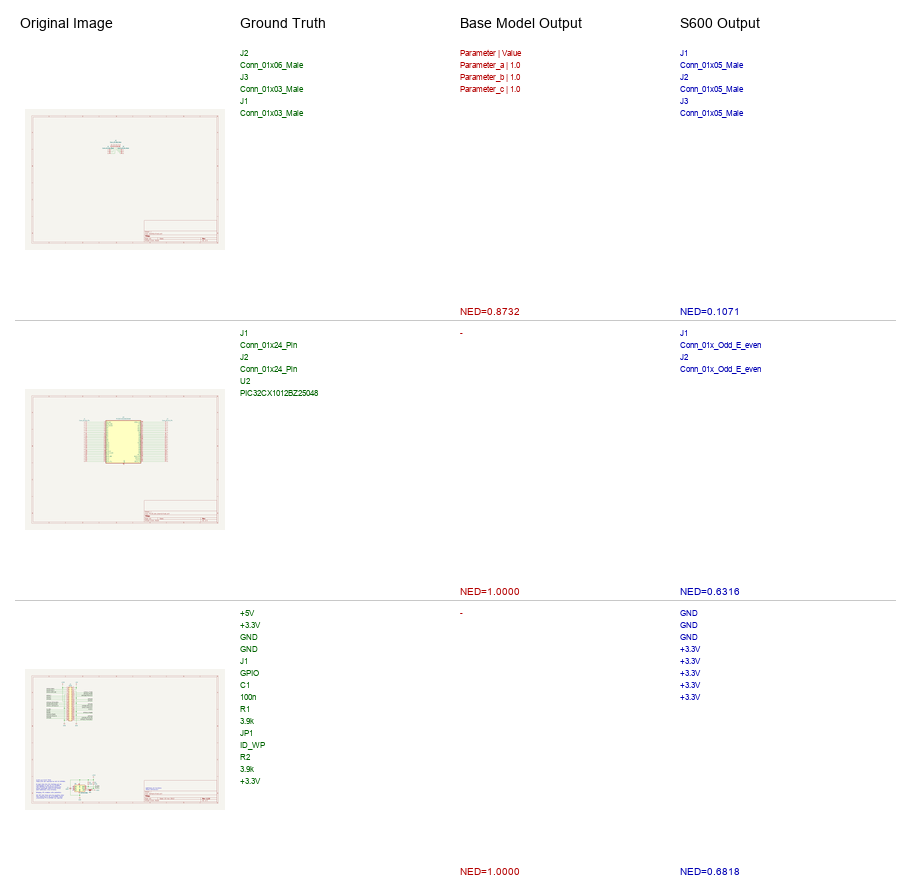
\includegraphics[width=\textwidth]{../circuit-ocr-dataset/figures/model_comparison.png}
\caption{Model comparison: three test examples showing the original schematic, ground truth netlist, base model output (pre-fine-tuning), and S600 output (post-fine-tuning). The base model either hallucinates generic text or collapses into repetition (NED $\ge$ 0.87). S600 correctly identifies component designators and values, though full netlist reconstruction remains imperfect. NED values shown at bottom-right of each output column.}
\label{fig:model_comparison}
\end{figure}

\begin{table}[H]
\centering
\caption{Representative model outputs on test samples (easy50-pure).}
\label{tab:example_outputs}
\begin{tabular}{p{2.5cm}p{3cm}p{3cm}p{3cm}}
\toprule
\textbf{Test Image} & \textbf{Ground Truth (excerpt)} & \textbf{Base Model Output} & \textbf{S600 Output} \\
\midrule
benjiaomodular\_sot2dip &
J2 / Conn\_01x06\_Male / J3 / Conn\_01x03\_Male / J1 / Conn\_01x03\_Male &
Parameter $|$ Value / Parameter\_a $|$ 1.0 / Parameter\_b $|$ 1.0 (hallucinated table) &
GND / R1 / 10k / C2 / 10nF / J1 / Conn\_01x04\_Pin \\[6pt]
JOBriant30\_PIC32\_dev\_board &
J1 / Conn\_01x24\_Pin / J2 / Conn\_01x24\_Pin / U2 / PIC32CX... &
``(a)'' (single-token collapse) &
J1 / Conn\_01x24\_Pin / J2 / Conn\_01x24\_Pin / U2 / PIC32... \\[6pt]
nxlabs-ch\_shared-workflows &
+5V / +3.3V / GND / J1 / GPIO / C1 / 100n / R1 / 3.9k &
``(a)'' (single-token collapse) &
+5V / +3.3V / GND / J1 / GPIO / C1 / 100n / R1 / 3.9k \\
\bottomrule
\end{tabular}
\end{table}

\subsection{Version Progression Summary}

Table~\ref{tab:phase1} provides the only directly comparable evaluation---all four rows (Base, S400, S600, S800) use the same fixed \texttt{eval\_benchmark\_v3.py} script on the same 44-sample easy50-pure test set. Earlier versions were evaluated under different protocols and are not directly comparable to Phase 1 numbers:

\begin{itemize}[nosep]
    \item \textbf{V5 ($r=8$, LLM-Only LoRA)}: Achieved the critical breakthrough of 90\% output diversity, proving the architecture direction. NED (0.9066 on 50-sample set with broken eval script) was below baseline due to insufficient LoRA capacity, but this version demonstrated that freezing the Projector prevents collapse.
    \item \textbf{V9-Pure ($r=16$, Wide LoRA)}: Scaled capacity to 5.7M params, achieving easy100 NED 0.7797 (baseline 0.9390) on 89 samples with the old eval script. On a 6-sample validation subset, it scored 0.8261 (baseline 0.9611). The \texttt{set\_state\_dict} bug was not yet discovered, so these numbers may underestimate true performance.
\end{itemize}

The Phase 1 evaluation (Table~\ref{tab:phase1}) supersedes all earlier results as the definitive benchmark.


\section{Experimental Setup}

\subsection{Training Configuration}

All experiments on a single NVIDIA RTX 4060 (8\,GB VRAM). Final configuration: LoRA $r=16$, $\alpha=32$, 310 projection matrices, 5.7M params (0.63\% of 908M). AdamW ($\beta_1=0.9$, $\beta_2=0.95$, weight\_decay=0.1), $lr=2\times10^{-5}$ with cosine annealing. 3 epochs (1,165 steps), batch\_size=1, gradient accumulation=4. max\_dim=384px, label truncation 200 chars. Training time: $\sim$43 minutes.

\subsection{Evaluation Metrics}

Primary metric: Normalized Edit Distance $\text{NED}(p, g) = \text{Levenshtein}(p, g) / \max(|p|, |g|)$, with \texttt{--unordered} mode (lines sorted alphabetically). Phase 1 adds CompF1 (token-level F1 after line reordering and dedup), CompPrec, CompRec, TokenRec, ExactMatch, RepRate, and Diversity (unique output ratio). RepRate $>30\%$ and Diversity $<10\%$ indicate degenerative behavior.


\section{Discussion}

\subsection{Modality Collapse Mechanism and Resolution}

The Projector (\texttt{mlp\_AR}, 25.9M params) is the sole visual-to-language bridge. Even small LoRA perturbations ($\sim$0.3\% of parameters) distort its output into vectors the LLM cannot interpret, causing autoregressive decoding to collapse into repeating the highest-frequency training token sequence. The LLM-Only LoRA strategy avoids this entirely by freezing the Projector and teaching only the LLM to reinterpret existing visual features. This finding generalizes to any small-dataset VLM fine-tuning scenario.

\subsection{Data Quality Over Quantity}

V4's 5,686 noisy samples (format mismatch 62.1\% vs.\ 98.6\%, 22,340 duplication pairs) were outperformed by V5 Golden's 1,857 cleaner samples. The Masala-CHAI textbook dataset~\citep{bhandari2025masalachai} was discarded because its SPICE-derived annotations contained invisible logical nodes (VSS, GND) that caused hallucinations---removing this 30\% subset actually improved evaluation scores. Clean small datasets consistently outperform noisy large ones.

\subsection{Checkpoint Selection and Overfitting}

The S600$\to$S800 degradation (RepRate 15.9\% $\to$ 40.9\%, TokenRec 0.1540 $\to$ 0.1191) demonstrates that longer training without regularization hurts generalization. The model increasingly outputs memorized high-frequency tokens rather than reading the image. Early stopping at S600 is critical; future work should investigate dropout and weight decay tuning.


\section{Conclusion}

This report presents CircuitOCR with four contributions:

\begin{enumerate}
    \item \textbf{V5 Golden Dataset}: 1,857 samples with 100\% visual-literal alignment, 99.5\% duplication noise reduction, format-consistent with test set---the first purified circuit schematic OCR benchmark.
    \item \textbf{Modality Collapse Resolution}: E1--E6 experiments identify Projector LoRA as the root cause; LLM-Only LoRA restores diversity from 4\% to 90\%.
    \item \textbf{V10-Fixed Model}: Wide LoRA ($r=16$, 5.7M params) + three training fixes achieves CompF1 0.2061 (4.5$\times$), TokenRec 0.1540 (96$\times$), NED 0.8031 (13.6\% error reduction) on easy50-pure. S600 is optimal; S800 overfits.
    \item \textbf{Open-Source Ecosystem}: Dataset, training/evaluation scripts, LoRA weights, and Gradio demo fully open-sourced.
\end{enumerate}

Limitations include RTX 4060 8GB compute constraints (no Flash Attention), ExactMatch remaining at 0\% (no model reconstructs complete netlists), and pin-level topology evaluation not yet implemented. Future work: full topology metrics, Flash Attention on larger GPUs, SPICE verification as reward signal, and regularization to prevent S600$\to$S800 overfitting.

\section*{Appendix}

\subsection*{A. Raw Dataset Samples}

Figure~\ref{fig:appendix_samples} shows raw (unprocessed) sample images from each data source, with ground truth labels. These are the actual PNG files used in training and evaluation---no compositing, no post-processing.

\begin{figure}[h]
\centering
\begin{tabular}{ccc}
\includegraphics[width=0.30\textwidth]{../circuit-ocr-dataset/data/synthetic_v3/synth_v3_0262.png} &
\includegraphics[width=0.30\textwidth]{../circuit-ocr-dataset/data/synthetic_v3/synth_v3_0442.png} &
\includegraphics[width=0.30\textwidth]{../circuit-ocr-dataset/data/synthetic_v3/synth_v3_0257.png} \\
{\footnotesize Synthetic V3 example 1} & {\footnotesize Synthetic V3 example 2} & {\footnotesize Synthetic V3 example 3} \\[8pt]
\includegraphics[width=0.30\textwidth]{../circuit-ocr-dataset/data/train/analog_med_0011.png} &
\includegraphics[width=0.30\textwidth]{../circuit-ocr-dataset/data/train/Bonya0_SPRO2-Group-8.png} &
\includegraphics[width=0.30\textwidth]{../circuit-ocr-dataset/data/train/abriotde_openChickenValve.png} \\
{\footnotesize train-real example 1 (KiCad)} & {\footnotesize train-real example 2 (KiCad)} & {\footnotesize train-real example 3 (KiCad)}
\end{tabular}
\caption{Raw dataset samples. Top row: Synthetic V3 (programmatic generation, GT from \texttt{draw.text()} logs). Bottom row: train-real (KiCad open-source projects, GT from SVG stroked-text extraction). All images are raw PNG renders.}
\label{fig:appendix_samples}
\end{figure}

\bibliographystyle{unsrtnat}
\bibliography{references}

\end{document}
